\documentclass{article}
\usepackage[utf8]{inputenc}
\usepackage{amsmath}
\usepackage{fullpage}
\usepackage{multicol}
\usepackage{natbib}
\usepackage{graphicx}
\usepackage{subfig}
\usepackage{caption}
\usepackage{subcaption}
\usepackage{verbatim}
\usepackage[hungarian]{babel}

\newcommand\ddfrac[2]{\frac{\displaystyle #1}{\displaystyle #2}}

\captionsetup{justification=centering}

\title{onallo project II Kis Adam}
\author{aregic}
\date{March 2018}

\begin{document}
\maketitle

\section{Introduction}

\begin{multicols}{2}

Methods tryed:
\begin{itemize}
    \item bounding box instead of bounding polygon
\end{itemize}

\end{multicols}

\section{Példahalmaz növelése}
A mélytanulásos módszerek egyik nagy gyengesége jelenleg, hogy a betanításhoz nagy példahalmazra van szükség, azonban a képek felcímkézése nagyon drága, mert nem (jól) autómatizálható. A feladathoz eredetileg 499 db példát kaptam. Összehasonlításképpen, az ImageNet adatbázis, amin a mélytanulási módszereket össze szokták hasonlítani több mint 14 millió képet tartalmaz \cite{imagenet_database}, bár kategóriánként nagy az eltérés, ezertől százezerig. Hosszabb keresgélés után az Ade 20k adathalmazt találtam, ami könnyen hozzáférhető (nem kutatóknak is)\cite{ade20k_database}. Ez szegmentálásos feladatra lett kitalálva: minden képponthoz meg van adva, hogy milyen tárgyhoz tartozik (ház, autó...). Van egy nagy előnye, amit jelenleg nem használok ki, hogy tárgyak részeit is külön kategorizálja: egy képpont tartozhat egyszerre egy autóhoz és azon belül egy rendszámtáblához, vagy egy házhoz és azon belül egy ablakhoz.

Ezzel együtt a tanító halmazom 1258 darabra bővült, az ellenörző halmazom 536-ra (CHECK!!!). Ennek azonban megvan az az ára, hogy ezt a példahalmazt nem kifejezetten erre a feladatra találták ki, ezért a rendszámok legtöbbször nem leolvashatóak és a felvételek szemszöge sem egyezik meg az ellenörző kamerák tipikus szemszögével: a képek fejmagasságból lettek készítve, míg az ellenörző kamerák tipikusan 4-5 méter magasságban vannak (\ref{fig:orig_dataset_example}. ábra). Ez jelentheti azt, hogy a háló nem lesz képes más szemszögből készült képeken felismerni a rendszámtáblákat, de azt is, hogy a két példahalmaz egyesítésével rá lesz kényszerítve, hogy elvonatkoztasson a nézőponttól. Másik probléma, hogy a rendszámok sokszor (bár nem mindig) kivehetetlenek. Ez az előzőhöz hasonlóan segíthet, hogy más jelekből ismerje fel a rendszámtáblát, például az autó pozícióját felhasználva, de mind a két probléma a felé mutat, hogy a betanulás hosszabb és nehezebb lesz, ha egyáltalán (adott erőforrások mellett), lehetséges. Ha a cél az eredeti példahalmazon való jó eredmény elérése, akkor ezeken betanítva a hálónak jobb eredményt kellene produkálnia, mert arra motiválja, hogy ne csak részletek alapján ismerje fel, hanem legalább egy primitív modellt építsen fel az autóról és annak valószínű pozícióiról. A betűk felismerése önmagában hibát hordoz: lehetséges, hogy a betűk egy utcatáblán vannak (bevallom egy ilyennel sem találkoztam, de a lehetőség fennáll), de az eredeti példahalmazban vannak arab rendszámok is, amik tovább komplikálják a betűk felismerését. Egy további hiba, hogy az új adathalmazban nincsenek motorosok, míg az eredetiben igen.

\begin{figure}[h!]%
    \centering
    \subfloat[Kép az eredeti példahalmazból]{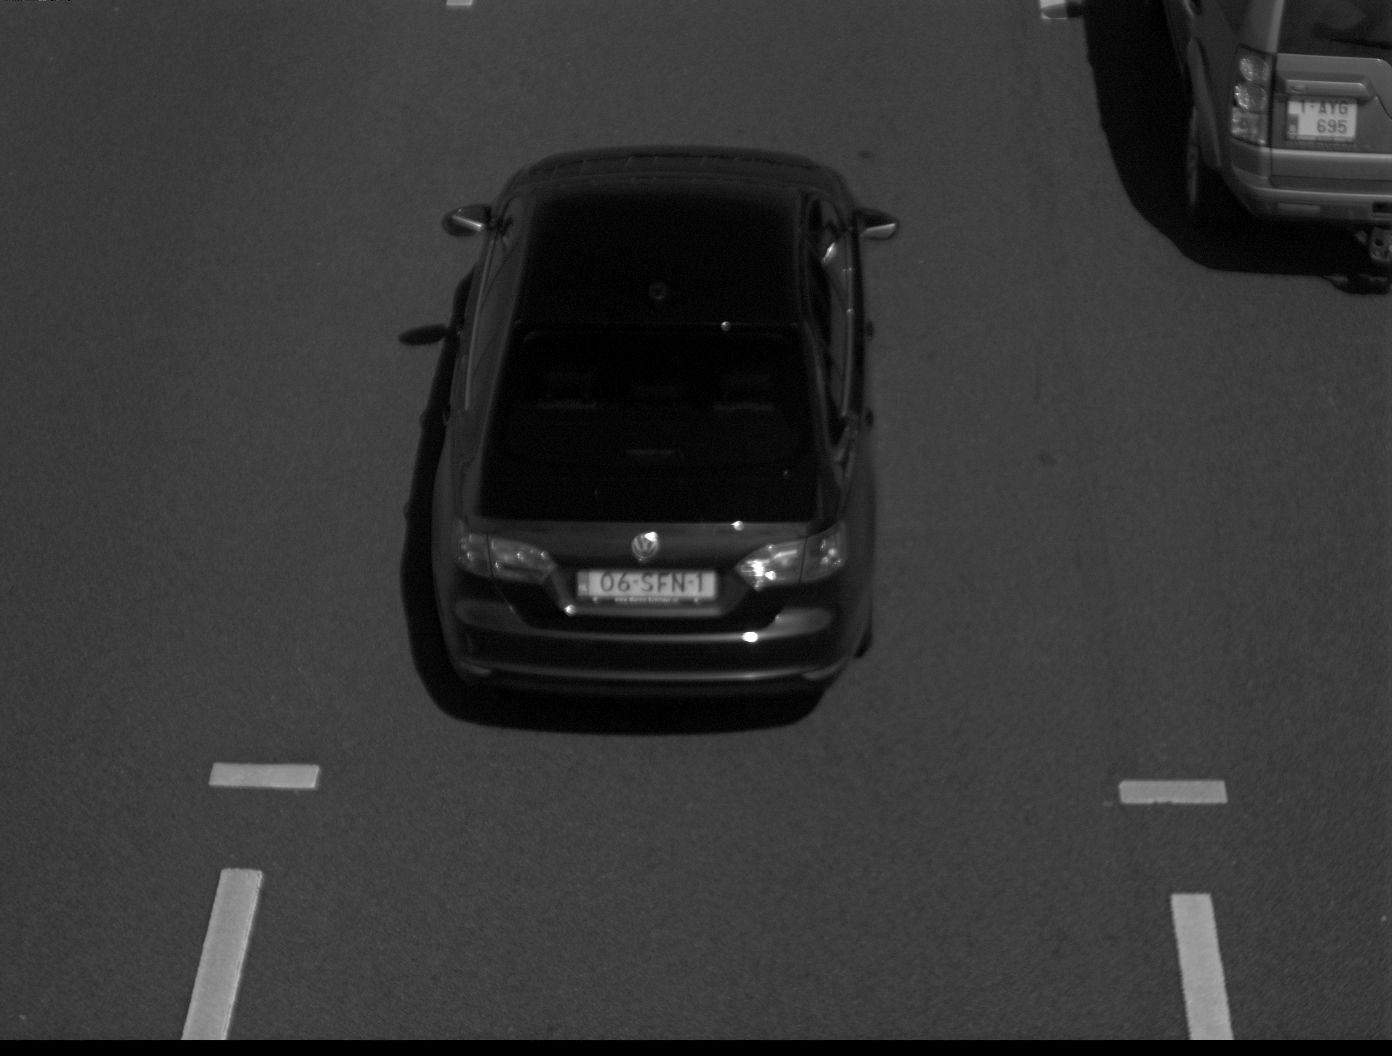
\includegraphics[width=.4\linewidth]{original_dataset_example.jpg}}%
    \qquad
    \subfloat[ADE 20k dataset egy eleme]{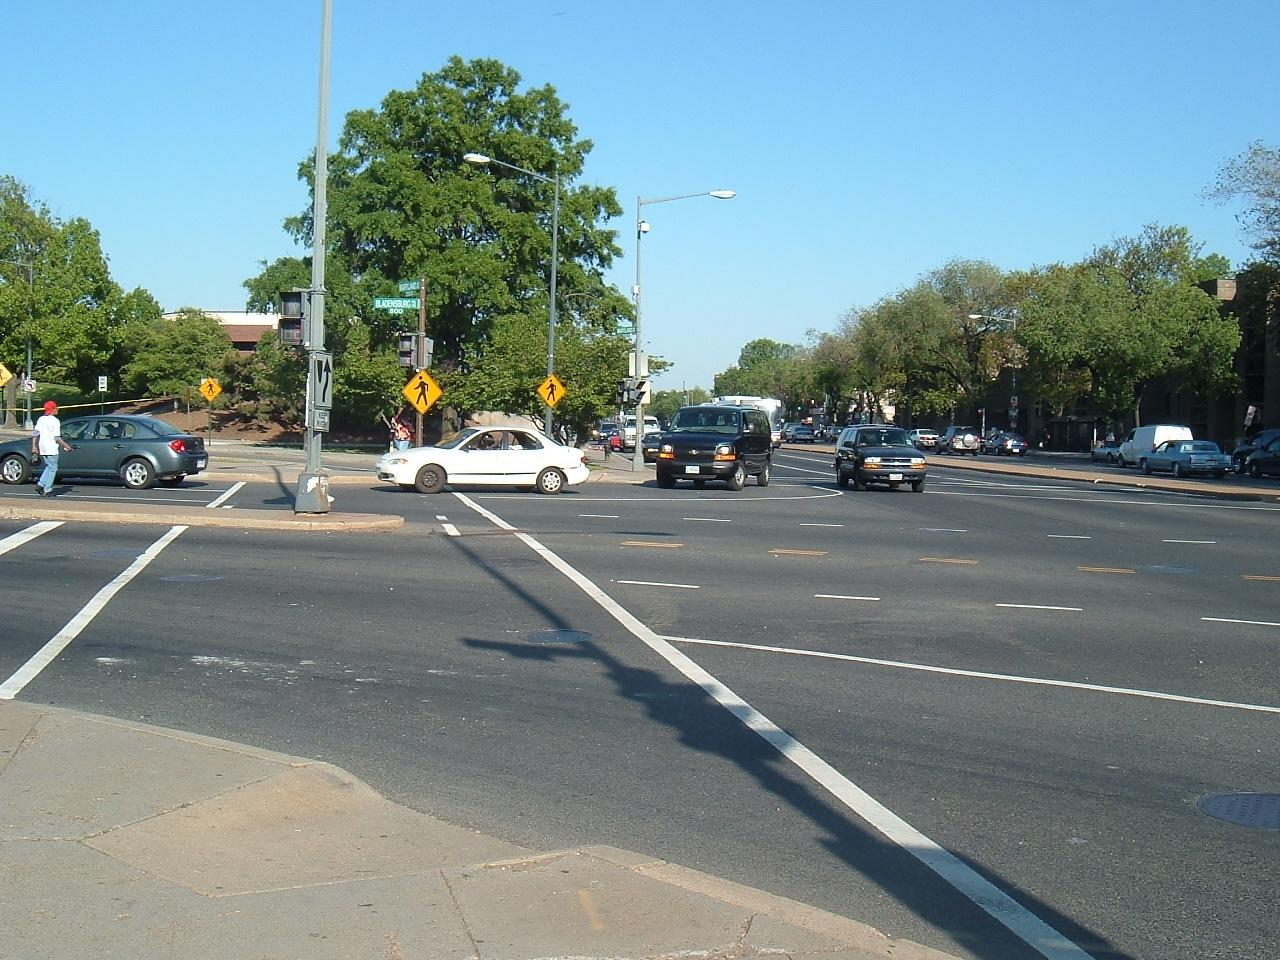
\includegraphics[width=.4\linewidth]{ADE_train_sample.jpg}}%
    \centering
    \caption{Az eredeti példahalmazban a kép tipikusan felülről készült (szög eltérő), az újban azonban fejmagasságból. Másik probléma, hogy a (b) képen a rendszám alig látszik és nem is leolvasható.}%
    \label{fig:orig_dataset_example}%
\end{figure}

\begin{figure}[h!]
    \centering
    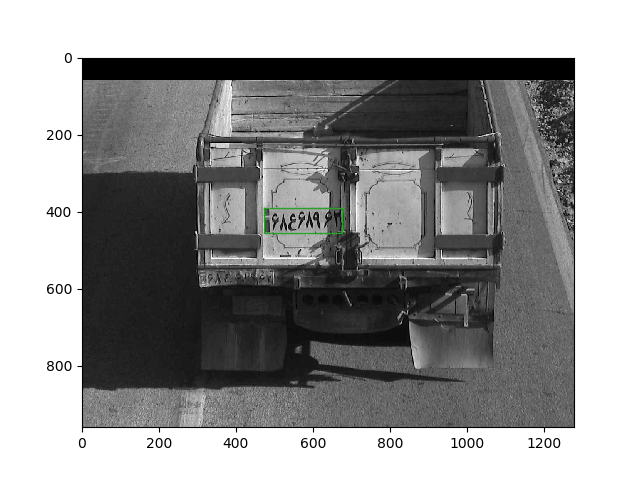
\includegraphics[scale=1.0]{difficult_example_orig_dataset.png}
    \caption{Egy nehéz példa: a rendszám árnyalata alig tér el az környezetétől (színesben egy kicsit jobban), a betűk kézzel lettek felfestve és az arab ábct használja}
    \label{fig:difficult_example}
\end{figure}

\section{Eltűnő/felrobbanó gradiens}
A mélytanulásban egy általános probléma, hogy a visszaterjesztés során a gradiens egyre kisebb vagy nagyobb lesz. Ennek a végeredménye, hogy az alsőbb rétegekben a gradiens értéke vagy túl nagy lesz, vagy elenyészően kicsi.

Tegyük fel, hogy a háló $n$ rétegből áll. Jelölje $w_i$ az i. réteg paramétereinek vektorát. Tegyük fel, hogy létezik $0 < b < 1$ szám, hogy $\forall i \  ||\nabla (w_i)||_{\infty} < b$. Ekkor $||\nabla (w_i)||_{\infty} < b^{(n-i+1)}$, speciálisan $||\nabla (w_1)||_{\infty} < b^n$. Ha ez a $b$ kellően kicsi, akkor az első rétegbeli gradiensek elenyészőek lesznek, akár számítási hibán belüliek is, azaz a gradiens (vagy ellentetje) hozzáadása a súlyhoz semmilyen változást nem fog okozni. Ekkor az alsó rétegek nagyon lassan, vagy akár egyáltalán nem tanulnak. Ha ezt magas \textit{learning rate}-tel akarjuk ellensúlyozni, akkor a felsőbb rétegek súlyai túl nagyokat ugrálhatnak, amíg az alsók alig mozognak, . Ennek ellentéte a felrobbanó gradient, amikor $\exists b > 1 \ \forall i \  ||\nabla (w_i)||_{\infty} > b$. Ekkor  $||\nabla (w_i)||_{\infty} > b^{(n-i+1)}$, speciálisan $||\nabla (w_1)||_{\infty} > b^n$. Ez általában gyorsan ahhoz vezet, hogy az alsó réteg súlyai közül sok értéke \textit{NaN} lesz és a háló nem ad értelmezhető kimenetet.

Ennek elkerülésére több megoldás létezik. A ReLU aktivációs függvény sikerét sokat pont annak tulajdonítják, hogy elkerüli a \textit{szigmoid szaturáció} problémáját \cite{krizhevsky2012imagenet}. Ez azonban csak az aktivációs függvényből adódó eltűnő gradiens problémát oldja meg, de az adódhat a súlyok értékéből is.

\section{Neuron kimenetének normalizálása}

LeCunn megmutatta, hogy a tanulás sebességében segít, hogy ha a neuron kimenetének varianciája 1 körül van\cite{lecun1998efficient}. Ennek oka eredetileg a szigmoid szaturáció volt, de ReLU aktivációs függvény esetében is segít. Ennek elérésére 2 megoldást alkalmaztam:

\begin{itemize}
    \item Glorot (vagy Xavier) inícializáció \cite{glorot2010understanding}
    \item Batch normalization \cite{fcholl_batch_norm_szegedy}
\end{itemize}

\subsection{Glorot inícializáció}

A cél úgy inícializálni, hogy a varianciája a neuronok bemenetének 1 legyen. Mivel két 1 szórású, 0 várható értékű, független változó szorzatának 1 a várható értéke:

\begin{equation}
    \text{Var}(XY) = \text{E}(X^2)\text{E}(Y^2) - [\text{E}(X)]^2 [\text{E}(Y)]^2 = 1 - 0 = 1
\end{equation}

és két független eloszlású változó varianciája egyszerűen a varianciájuk összege, ezért ha induláskor a neuronok kimenetét függetlennek vesszük, akkor egy adott neuron egy bemenetének varianciája:

\begin{equation}
    \text{Var}(x) = n\text{Var}(f)
\end{equation}

Ahol $n$ a bemenetek száma, Var$(f)$ az előző réteg kimenetének varianciája (itt felteszem, hogy mindre azonos, ezért nem fontos, hogy $f$ melyik alatta lévő neuront jelöli). $f$ itt egy leaky ReLU kimenete:

\begin{equation}
    f(x) = \left\{
        \begin{array}{ll}
            x       & \text{ha}\ x > 0 \\
            0.1x    & \text{különben}
        \end{array}
    \right.
\end{equation}

Azaz ha E$[x] = 0$, akkor
\begin{equation}
    \text{Var}(f) = \ddfrac{\text{Var}(x) + 0.1\text{Var}(x)}{2}
\end{equation}

Ezt szeretnénk, ha 1 lenne, azaz:

\begin{equation*}
    \ddfrac{\text{Var}(x) + 0.1\text{Var}(x)}{2} = 1
\end{equation*}
\begin{equation*}
    \text{Var}(x) = \ddfrac{2}{1.1}
\end{equation*}

De Var$(x) = \text{Var}(\sum w_i x_i)$. Felételezve, hogy $x_i$ varianciája 1, átlaga 0, és feltételezve hogy $w_i$-k átlaga 0, varianciája 1, továbbá függetlenek:
\begin{equation*}
    \text{Var}(w_i) = \ddfrac{2}{1.1n}
\end{equation*}

Ahol $n$ az $x$ bemeneteinek száma. Az eredeti publikációnak megfelelően normál eloszlást választottam \cite{glorot2010understanding}:
\begin{equation*}
    w_i \sim \mathcal{N}(0, \frac{2}{1.1n})
\end{equation*}

\subsection{Ortogonális inícializáció}

Nyilvánvaló, hogy ha két neuron kimenete lineárisan összefüggő, akkor az egyiket feleslegesen számoltuk ki: ha $f_1$ az egyik kimenet, $f_2$ a másik és $f_2 = \lambda f_1$, akkor a rákövetkező rétegben $w_1 f_1 + w_2 f_2 = (w_1 + \lambda w_2)f_1$. Emiatt segít, hogy ha a súlyokat ortogonálisra inícializáljuk, amennyire csak lehetséges. Mivel a konvolúció (vagy pontosabban kereszt korreláció) gyakorlatilag skaláris szorzatok sorozata, a súlyok mátrix alakja megtévesztő: valójában inkább vektorokként érdemes kezelni őket, azaz egy 3x3 konvolúciós mátrix felfogható egy 9 elemből álló vektorként. Nyilván ekkor pontosan 9 ortogonális vektort képezhetünk, de ez csak a mátrix (vagyis inkább vektor) méretétől függ. Ezzel a módszerrel valamennyire továbbfejleszthető az eredeti Glorot inícializáció. Legyen $n$ db konvolúciós kernel egy rétegben, ezek mérete legyen $m \times m$-es. Ekkor az algoritmus:
\begin{itemize}
    \item Vegyünk $n$ db vektort, aminek eloszlása $\mathcal{N}(0, 1)$
    \item Ortogonalizáljuk SVD algoritmussal
    \item Szorozzuk meg a kapott mátrixot $\frac{2}{1.1n}$-nel
\end{itemize}

Amennyiben $m^2 \ge n$, a kapott súlyok páronként ortogonálisak lesznek és varianciájuk $\frac{2}{1.1n}$ lesz, ami megfelel a fentebbi, Glorot inícializáció során támasztott követelménnyel. Tesztjeim során azt kaptam, hogy ez jelentősen javítja a konvergenciát a tanulás kezdeti szakaszában.

KÉPET ERRŐL!!!

Ennél vannak komplexebb módszerek is \cite{mishkin2015all}, amelyeket érdemes a jövőben megvizsgálni. Dmytro Mishkin benchmark-ja szerint valamivel jobban konvergál \cite{ducha-aiki-caffenet-batch-norm-benchmark}.


\subsection{Gábor wavelet}

Egy érdekes eredménye az AlexNet publikációnak\cite{krizhevsky2012imagenet}, hogy az első réteg konvolúciós kernele a tanítás végére Gábor-wavelet-hez hasonlóvá vált:

\begin{figure}[h!]
    \centering
    \includegraphics[scale=1.0]{alexnet-first-layer.png}
    \caption{A publikációban szereplő első réteg konvolúciós kerneleinek vizualizációja. A fehér-fekete csíkok hasonlítanak a Gábor wavelet-ekre.}
    \label{fig:difficult_example}
\end{figure}

A Gábor wavelet-ek használata a képfeldolgozásban nem újkeletű \cite{541406}, és macskák vizuális kérgének bizonyos része is jól közelíthető vele. Kipróbáltam, hogy az alsó réteget úgy inícializálom, hogy ezeket is tartalmazza, meg pár sima élkeresőt illetve kört. Az élkeresőhöz is Gauss ablakot raktam (Scharr operátor), amiatt, mert jól reprezentálja mi a fontos a képfeldolgozás során: az érdekel elsősorban minket, hogy egy pont környezetében él van-e, de attól távolodva a pontok világosságértéke egyre kevésbé fontos, így kevésbé szabályos éleket is meg tud találni.

KÉPET

A kísérleteim eredménye azonban, hogy ezek nem segítettek. A hiba, hogy ehhez viszonylag nagy méretű kernelekre van szükség, ráadásul a legalsó rétegben, ahol a \textit{max pooling} rétegek még nem húzták össze a képet, azaz itt a konvolúció számítási igénye még nagyon magas. Ha a kép $700 \times 700$ képpontból áll, akkor a $n \times n$ kernellel való ú.n. SAME konvolúció $700 \times 700 \times n \times n$ szorzást igényel és $700 \times 700 \times (n \times n - 1)$ összeadást. Ez nagyon drága, ráadásul nem túl rugalmas: nem tudja pl. egykönnyen lecserélni a kernel bal alsó sarkát. Ha ehelyett mondjuk hozáadunk plusz egy réteget, az már képes erre. Ennek következményeként jobb $3 \times 3$-as kerneleket használni az alsó rétegben és a felszabaduló kapacitást több réteg hozzáadására költeni. Fast YOLO \cite{redmon2016you} is inkább ezt a megoldást használja.

\begin{comment}
    A visszaterjesztéses tanulás alapja a deriválás lánc-szabálya. Legyen a $w_i$  egy neuron súlyainak $n$ dimenziós vektora, $x_i$ egy adott bemeneti vektor, $b_i$ pedig az eltolásvektor. Ekkor az i. neuron kimenete:
    
    \begin{equation}
        f_i = \text{ReLU}(\sum_{j=1}^{n}w_{i,j} x_{i,j} + b_{i,j})
    \end{equation}
    
    Itt Leaky ReLU-t használok, ami emlékeztetőnek:
    \begin{equation}
        \phi(x) = \left\{
            \begin{array}{ll}
                x       & \text{ha}\ x > 0 \\
                0.1x    & \text{különben}
            \end{array}
        \right.
    \end{equation}
    
    
    Tegyük fel, hogy $f_i$ kimeneti meuron, $x_i$ egy másik neuron kimenete. Legyen ez a neuron az $f_{i-1}$. Itt én Leaky ReLU-t használok, azaz egy $w_{i-1}$ súlyra vett parciális derivált:
    
    \begin{equation}
        \begin{array}{ll}
            \ddfrac{\partial f_i}{\partial w_{i-1}} = x_{i-1} w_i & \text{ha } \sum_{i=1}^{n}w_{i-1,j} x_{i-1,j} + b_{i-1,j} \ge 0 \\
            \\
            \ddfrac{\partial f_i}{\partial w_{i-1}} = 0.1 x_{i-1} w_i & \text{ha } \sum_{i=1}^{n}w_{i-1,j} x_{i-1,j} + b_{i-1,j} < 0
        \end{array}
    \end{equation}
    
    Vagyis a súlyra vett derivált értéke függ a következő réteg súlyaitól. Ha még egy réteggel visszaterjesztjük (az egyszerűség kedvéért tegyük fel, hogy minden neuron kimenete pozitív, mert ekkor a leaky ReLU deriváltja 1):
    
    \begin{equation}
            \ddfrac{\partial f_i}{\partial w_{i-2}} = \ddfrac{\partial f_i}{\partial f_{i-1}} \ddfrac{\partial f_{i-1}}{\partial w_{i-2}} = 
                x_{i-2} w_{i-1} w_i \\
    \end{equation}
    
    És így tovább. Egy neuron kimenete azonban több neuronhoz van kapcsolva a következő rétegben, így a végső gradiens a tagonkénti deriválás szabályának megfelelően az ezekre vett parciális deriváltak összege.
    
    A célunk, hogy a súlyokra vett parciális deriváltak átlagos 1 közelében legyenek, mert ekkor a súlyok megközelítőleg azonos mértékben változnak a tanulás során. 
    
    \begin{equation}
        \text{Error}' = 2(f_n - l)f'
    \end{equation}

\end{comment}

\section{Sample augmentation}
\begin{itemize}
    \item random cropping
    \item Gauss zaj
\end{itemize}

\section{Batch normalization}

A batch normalizálást közvetlenül a ReLU előtt vagy után érdemes rakni. Christian Szegedy eredetileg a ReLU előtt használta \cite{ioffe2015batch}, később áttért arra, hogy utána, de a kérdés messze nem eldöntött \cite{fcholl_batch_norm_szegedy}.

Gradiensek batch normalizálással:

\begin{center}
\begin{tabular}{|c|c|}
	 \hline
		conv1/weights & 0.0009292062604799867 \\ 
		conv1/biases & 0.0011252182302996516 \\ 
		conv2/weights & 0.003921532072126865 \\ 
		conv2/biases & 0.0008371319272555411 \\ 
		conv3/weights & 0.01155342347919941 \\ 
		conv3/biases & 0.00041879608761519194 \\ 
		conv4/weights & 0.016506094485521317 \\ 
		conv4/biases & 0.00035374442813917994 \\ 
		conv5/weights & 0.02579069696366787 \\ 
		conv5/biases & 0.0014705421635881066 \\ 
		conv6/weights & 0.16252420842647552 \\ 
		conv6/biases & 0.001693260739557445 \\ 
		local3/weights & 0.5378696322441101 \\ 
		local3/biases & 0.0013500589411705732 \\ 
		tile\_output\_layer/weights & 0.11695990711450577 \\ 
		tile\_output\_layer/biases & 1.400262128470331e-10 \\ 
	\hline
\end{tabular}
\end{center}


\bibliographystyle{plain}
\bibliography{references}
\end{document}

